%%%%%%%%%%%%%%%%%%%%%%%%%%%%%%%%%%%%%%%%%
% Short Sectioned Assignment
% LaTeX Template
% Version 1.0 (5/5/12)
%
% This template has been downloaded from:
% http://www.LaTeXTemplates.com
%
% Original author:
% Frits Wenneker (http://www.howtotex.com)
%
% License:
% CC BY-NC-SA 3.0 (http://creativecommons.org/licenses/by-nc-sa/3.0/)
%
%%%%%%%%%%%%%%%%%%%%%%%%%%%%%%%%%%%%%%%%%

%----------------------------------------------------------------------------------------
%	PACKAGES AND OTHER DOCUMENT CONFIGURATIONS
%----------------------------------------------------------------------------------------

\documentclass[paper=a4, fontsize=11pt]{scrartcl} % A4 paper and 11pt font size

\usepackage{graphicx}
\usepackage[T1]{fontenc} % Use 8-bit encoding that has 256 glyphs
\usepackage{fourier} % Use the Adobe Utopia font for the document - comment this line to return to the LaTeX default
\usepackage[english]{babel} % English language/hyphenation
\usepackage{amsmath,amsfonts,amsthm} % Math packages

\usepackage{lipsum} % Used for inserting dummy 'Lorem ipsum' text into the template
\usepackage{algorithm}
\usepackage{algpseudocode}
\usepackage{sectsty} % Allows customizing section commands
\allsectionsfont{\scshape} % Make all sections centered, the default font and small caps

\usepackage{algorithm,algpseudocode}% http://ctan.org/pkg/{algorithms,algorithmx}
\algnewcommand{\Inputs}[1]{%
  \State \textbf{Inputs:}
  \Statex \hspace*{\algorithmicindent}\parbox[t]{.8\linewidth}{\raggedright #1}
}
\algnewcommand{\Initialize}[1]{%
  \State \textbf{Initialize:}
  \Statex \hspace*{\algorithmicindent}\parbox[t]{.8\linewidth}{\raggedright #1}
}

\usepackage{fancyhdr} % Custom headers and footers
\pagestyle{fancyplain} % Makes all pages in the document conform to the custom headers and footers
\fancyhead{} % No page header - if you want one, create it in the same way as the footers below
\fancyfoot[L]{} % Empty left footer
\fancyfoot[C]{} % Empty center footer
\fancyfoot[R]{\thepage} % Page numbering for right footer
\renewcommand{\headrulewidth}{0pt} % Remove header underlines
\renewcommand{\footrulewidth}{0pt} % Remove footer underlines
\setlength{\headheight}{13.6pt} % Customize the height of the header

\numberwithin{equation}{section} % Number equations within sections (i.e. 1.1, 1.2, 2.1, 2.2 instead of 1, 2, 3, 4)
\numberwithin{figure}{section} % Number figures within sections (i.e. 1.1, 1.2, 2.1, 2.2 instead of 1, 2, 3, 4)
\numberwithin{table}{section} % Number tables within sections (i.e. 1.1, 1.2, 2.1, 2.2 instead of 1, 2, 3, 4)

\setlength\parindent{0pt} % Removes all indentation from paragraphs - comment this line for an assignment with lots of text

%----------------------------------------------------------------------------------------
%	TITLE SECTION
%----------------------------------------------------------------------------------------

\newcommand{\horrule}[1]{\rule{\linewidth}{#1}} % Create horizontal rule command with 1 argument of height

\title{	
\normalfont \normalsize
\textsc{Rice University, Department of Computer Science} \\ [25pt] % Your university, school and/or department name(s)
\horrule{0.5pt} \\[0.4cm] % Thin top horizontal rule
\huge Assignment 5, COMP 540 \\ % The assignment title
\horrule{2pt} \\[0.5cm] % Thick bottom horizontal rule
}

\author{Chen Zeng(cz39), Zhihui Xie(zx18)} % Your name

\date{\normalsize\today} % Today's date or a custom date

\begin{document}

\maketitle % Print the title

\section{Deep neural networks}
\paragraph{\textbf{Answer1}}
In deep learning, part of the architecture of a deep network or part of the training process is typically devoted to unsupervised feature extraction. It can contain a great deal of information. Such data is clean enough and rich enough so that the nonlinear features learned by deep neural networks represent real phenomena within the data and are not just artifacts of over training. Shallow networks like single-layer network cannot own this feature due to the limitation of it's layer and parameters. Therefore, deep networks typically outperform shallow networks.
\\ ref: https://www.quora.com/When-should-I-prefer-deep-learning-algorithms-over-shallow-machine-learning-algorithms

\paragraph{\textbf{Answer2}}
Instead of the function being zero when x < 0, a leaky ReLU will instead have a small negative slope (of 0.01, or so). That is, the function computes $f\left ( x \right )=\begin{cases}
 x& \text{ if } x> 0 \\ 
 \alpha x& \text{ if } otherwise 
\end{cases}$ where $\alpha$ is a small constant.
\\ Leaky ReLUs are one attempt to fix the "dying ReLU" problem. ReLU units can be fragile during training and can "die". For example, a large gradient flowing through a ReLU neuron could cause the weights to update in such a way that the neuron will never activate on any datapoint again. If this happens, then the gradient flowing through the unit will forever be zero from that point on. That is, the ReLU units can irreversibly die during training since they can get knocked off the data manifold. 
\\ ref1: http://cs231n.github.io/neural-networks-1/
\\ ref2: https://en.wikipedia.org/wiki/Rectifier\_(neural\_networks)

\paragraph{\textbf{Answer3}}
Here are the contrast:
\begin{itemize}
  \item AlexNet
 	 \\ In 2012, AlexNet significantly outperformed all the prior competitors and won the challenge by reducing the top-5 error to 15.3\%. The second place top-5 error rate, which was not a CNN variation, was around 26.2\%.
  	\\ The network had a very similar architecture as LeNet by Yann LeCun et al but was deeper, with more filters per layer, and with stacked convolutional layers. AlexNet was trained simultaneously on two Nvidia Geforce GTX 580 GPUs which is the reason for why their network is split into two pipelines. AlexNet was designed by the SuperVision group, consisting of Alex Krizhevsky, Geoffrey Hinton, and Ilya Sutskever.
	\begin{figure}[H]
 		\centering
 		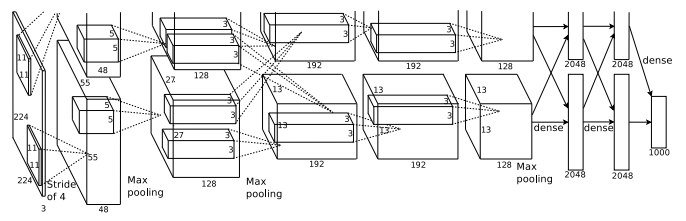
\includegraphics[scale=0.5]{./alexnet.png}
 		\caption{AlexNet}
 		\label{fig:alexnet}
 	\end{figure}
  \item VGG-Net
  	\\ The runner-up at the ILSVRC 2014 competition is dubbed VGGNet by the community and was developed by Simonyan and Zisserman . VGGNet consists of 16 convolutional layers and is very appealing because of its very uniform architecture. It only performs 3x33 times 33x3 convolutions and 2x22 times 22x2 pooling all the way through. It is currently the most preferred choice in the community for extracting features from images. The weight configuration of the VGGNet is publicly available and has been used in many other applications and challenges as a baseline feature extractor. However, VGGNet consists of 140 million parameters, which can be a bit challenging to handle.
	\begin{figure}[H]
 		\centering
 		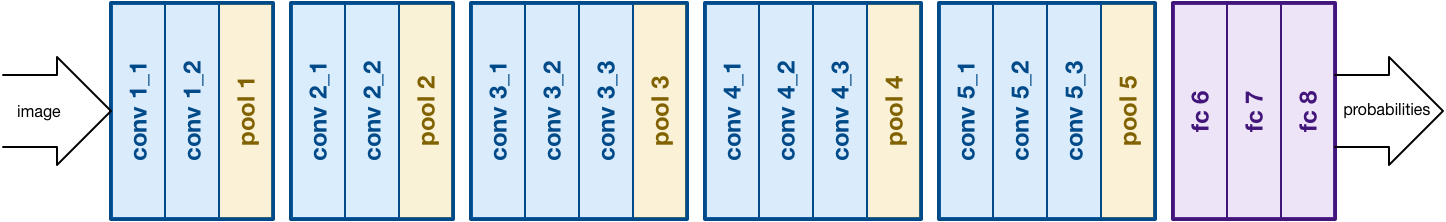
\includegraphics[scale=0.3]{./vggnet.png}
 		\caption{VGG-Net}
 		\label{fig:vggnet}
 	\end{figure}
  \item GoogleNet
  	\\ The winner of the ILSVRC 2014 competition was GoogleNet(Inception) from Google. It achieved a top-5 error rate of 6.67\%! This was very close to human level performance which the organisers of the challenge were now forced to evaluate. As it turns out, this was actually rather hard to do and required some human training in order to beat GoogLeNets accuracy. After a few days of training, the human expert (Andrej Karpathy) was able to achieve a top-5 error rate of 5.1\%. The network used a CNN inspired by LeNet but implemented a novel element which is dubbed an inception module. This module is based on several very small convolutions in order to drastically reduce the number of parameters. Their architecture consisted of a 22 layer deep CNN but reduced the number of parameters from 60 million (AlexNet) to 4 million.
	\begin{figure}[H]
 		\centering
 		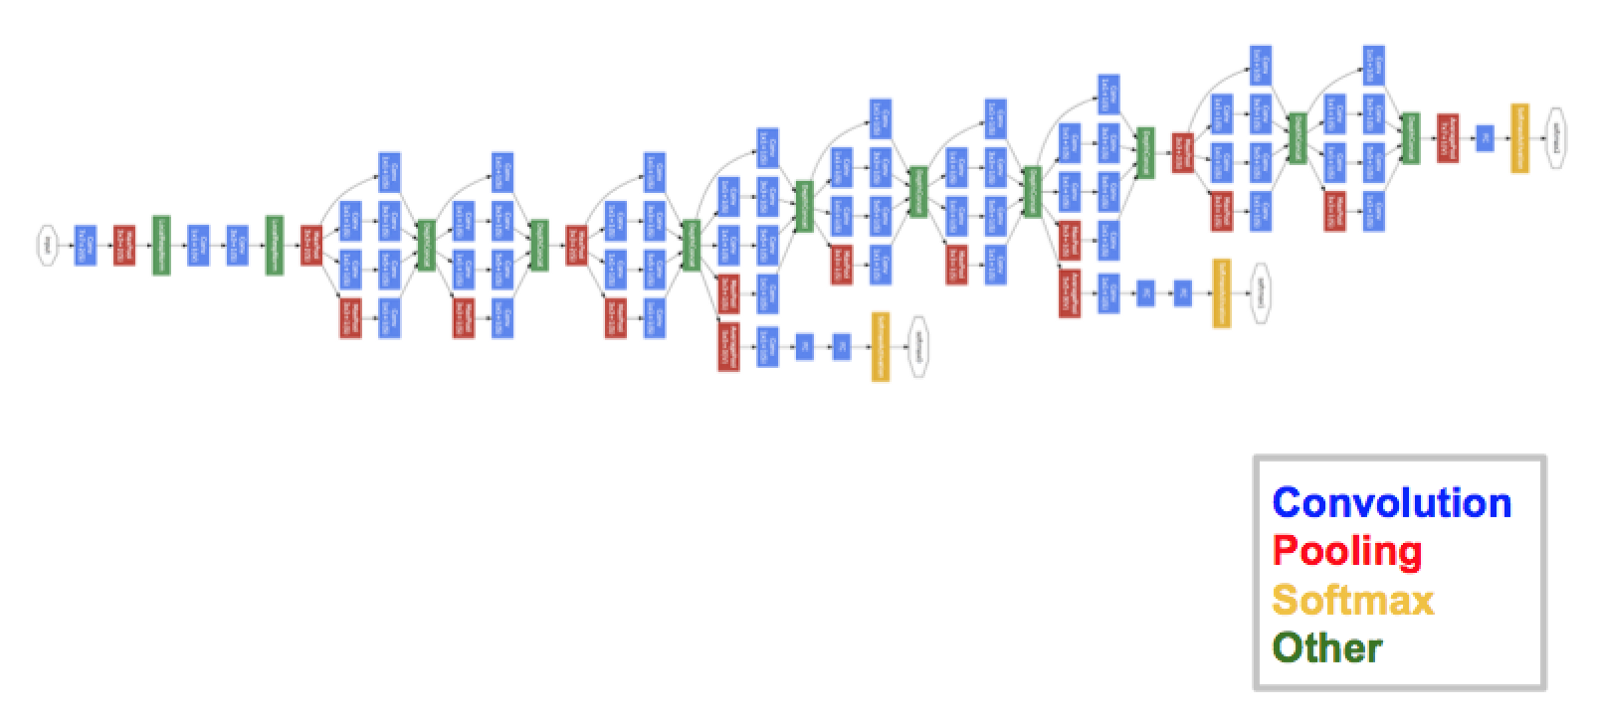
\includegraphics[scale=0.25]{./googlenet.png}
 		\caption{GoogleNet}
 		\label{fig:googlenet}
 	\end{figure}
  \item ResNet
  	\\ At last, at the ILSVRC 2015, the so-called Residual Neural Network (ResNet) by Kaiming He et al introduced anovel architecture with "skip connections" and features heavy batch normalization. Such skip connections are also known as gated units or gated recurrent units and have a strong similarity to recent successful elements applied in RNNs. Thanks to this technique they were able to train a NN with 152 layers while still having lower complexity than VGGNet. It achieves a top-5 error rate of 3.57\% which beats human-level performance on this dataset.
	\begin{figure}[H]
 		\centering
 		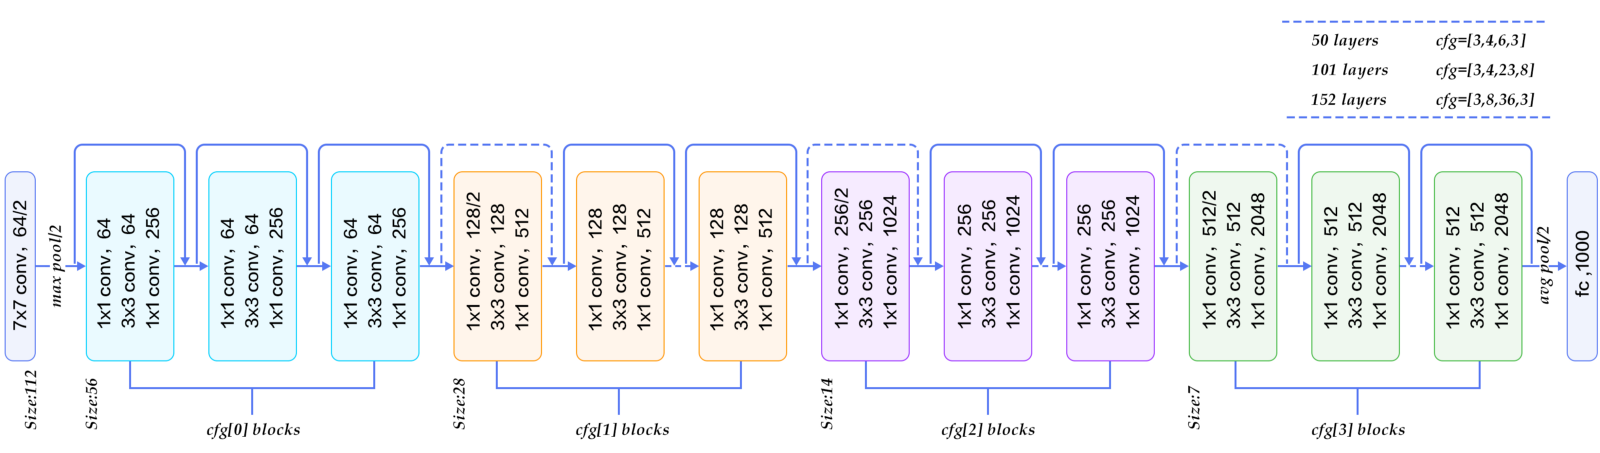
\includegraphics[scale=0.25]{./resnet.png}
 		\caption{ResNet}
 		\label{fig:resnet}
 	\end{figure}
\end{itemize}
Here are the one defining characteristic of each network:
\begin{itemize}
	\item AlexNet: the architecture is very similar to LeNet by Yann LeCun et al but was deeper
	\item VGG-Net: large amount of parameters which is about 140 million
	\item GoogleNet: reduced the number of parameters from 60 million (AlexNet) 
	\item ResNet: "skip connections" which is known as gated units or gated recurrent units
\end{itemize}
ref: https://medium.com/@siddharthdas\_32104/cnns-architectures-lenet-alexnet-vgg-googlenet-resnet-and-more-666091488df5

\section{Decision trees, entropy and information gain}
\paragraph{\textbf{Answer1}}
According to the definition of entropy, we have:
\begin{equation*}
H\left ( S \right )=-Slog\left ( S \right )-\left ( 1-S \right )log\left ( 1-S \right )
\end{equation*}
Take the derivation of it and then we can get:
\begin{equation*}
{H}'\left ( S \right )=\left ( -1-log\left ( S \right )+log\left ( 1-S \right )+1 \right )\left ( log\left ( e \right ) \right )=log\left ( \frac{1-S}{S}  \right ) log\left ( e \right )
\end{equation*}
At the same time, we know that $S=\frac{p}{p+n}$, which means it's range is $\left ( 0, 1 \right )$. Therefore, we have the range of ${H}'\left ( S \right )$ with the relationship of $q$ as below:
\begin{equation*}
{H}'\left ( S \right )=\begin{cases}
> 0 & \text{ if } 0<S<\frac{1}{2} \\ 
= 0 & \text{ if } S=\frac{1}{2} \\ 
< 0 & \text{ if } \frac{1}{2}<S<1 
\end{cases}
\end{equation*}
It proves that $H\left ( S \right )$ increase as $S$ increases from $0$ to $\frac{1}{2}$ and will decrease as $S$ increases from $\frac{1}{2}$ to $1$, which means $H\left ( S \right )$ will get the maximum as $S=\frac{1}{2}$. Therefore we can get:
\begin{equation*}
H\left ( S \right )\leq H\left ( \frac{1}{2} \right )=-\frac{1}{2}log\left ( \frac{1}{2} \right )-\left ( 1-\frac{1}{2} \right )log\left ( 1-\frac{1}{2} \right )=1
\end{equation*}
Thus $H\left ( S \right )\leq 1$ is proved.
\\ At the same time, according to the above discussion, $H = 1$ happens when and only when $S = \frac{1}{2}$, which means $\frac{p}{p+n} = \frac{1}{2}$. As we solve it, we find $p = n$.
\\ Thus $p = n$ when $H\left ( S \right ) = 1$ is proved.
\paragraph{\textbf{Answer2}}
Here are the calculation of the reduction in cost using misclassification rate, entropy, and Gini index for models A and B:
\begin{itemize}
	\item Using misclassification rate:
		\begin{equation*}
		cost\left ( D \right )=\frac{1}{\left | d \right |}\sum_{\left ( x,y \right )\in D}I\left ( y\neq y^{'} \right )
		\end{equation*}
		\begin{equation*}
		cost\left ( D \right )=\frac{1}{800}*400=\frac{1}{2}
		\end{equation*}
		As for model A:
		\begin{equation*}
		cost\left ( D_{left} \right )=\frac{1}{400}*100=\frac{1}{4}
		\end{equation*}
		\begin{equation*}
		cost\left ( D_{right} \right )=\frac{1}{400}*100=\frac{1}{4}
		\end{equation*}
		\begin{equation*}
		reduction_{A}=\frac{1}{2}-\frac{1}{2}*\frac{1}{4}-\frac{1}{2}*\frac{1}{4}=\frac{1}{4}
		\end{equation*}
		As for model B:
		\begin{equation*}
		cost\left ( D_{left} \right )=\frac{1}{800}*400=\frac{1}{2}
		\end{equation*}
		\begin{equation*}
		cost\left ( D_{right} \right )=\frac{1}{600}*200=\frac{1}{3}
		\end{equation*}
		\begin{equation*}
		reduction_{B}=\frac{1}{2}-\frac{3}{4}*\frac{1}{3}=\frac{1}{4}
		\end{equation*}
	\item Using entropy:
		\begin{equation*}
		cost\left ( D \right )=-\frac{400}{400+400}log\left ( \frac{400}{400+400} \right )-\frac{400}{400+400}log\left ( \frac{400}{400+400} \right )=1
		\end{equation*}
		As for the model A:
		\begin{equation*}
		cost\left ( D_{left} \right )=-\frac{300}{300+100}log\left ( \frac{300}{300+100} \right )-\frac{100}{300+100}log\left ( \frac{100}{300+100} \right )=0.8113
		\end{equation*}
		\begin{equation*}
		cost\left ( D_{right} \right )=-\frac{100}{300+100}log\left ( \frac{100}{300+100} \right )-\frac{300}{300+100}log\left ( \frac{300}{300+100} \right )=0.8113
		\end{equation*}
		\begin{align*}
		reduction_{A}&=cost\left ( D \right )-\frac{\left | D_{left} \right |}{\left | D \right |}cost\left ( D_{left} \right )-\frac{\left | D_{right} \right |}{\left | D \right |}cost\left ( D_{right} \right )
		\\ &=1-\frac{400}{800}*0.8113-\frac{400}{800}*0.8113
		\\ &=0.1887
		\end{align*}
		As for the model B:
		\begin{equation*}
		cost\left ( D_{left} \right )=-\frac{200}{200+400}log\left ( \frac{200}{200+400} \right )-\frac{400}{200+400}log\left ( \frac{400}{200+400} \right )=0.9183
		\end{equation*}
		\begin{equation*}
		cost\left ( D_{right} \right )=-\frac{200}{200+0}log\left ( \frac{200}{200+0} \right )-\frac{0}{200+0}log\left ( \frac{0}{200+0} \right )=0
		\end{equation*}
		\begin{align*}
		reduction_{B}&=cost\left ( D \right )-\frac{\left | D_{left} \right |}{\left | D \right |}cost\left ( D_{left} \right )-\frac{\left | D_{right} \right |}{\left | D \right |}cost\left ( D_{right} \right )
		\\ &=1-\frac{600}{800}*0.9183-\frac{200}{800}*0
		\\ &=0.311275
		\end{align*}
	\item Using Gini index:
		\begin{equation*}
		cost\left ( D \right )=2*\frac{400}{400+400}*\frac{400}{400+400}=\frac{1}{2}
		\end{equation*}
		As for the model A:
		\begin{equation*}
		cost\left ( D_{left} \right )=2*\frac{300}{300+100}*\frac{100}{300+100}=\frac{3}{8}
		\end{equation*}
		\begin{equation*}
		cost\left ( D_{left} \right )=2*\frac{100}{300+100}*\frac{300}{300+100}=\frac{3}{8}
		\end{equation*}
		\begin{align*}
		reduction_{A}&=cost\left ( D \right )-\frac{\left | D_{left} \right |}{\left | D \right |}cost\left ( D_{left} \right )-\frac{\left | D_{right} \right |}{\left | D \right |}cost\left ( D_{right} \right )
		\\ &=\frac{1}{2}-\frac{400}{800}*\frac{3}{8}-\frac{400}{800}*\frac{3}{8}
		\\ &=\frac{1}{8}
		\end{align*}
		As for the model B:
		\begin{equation*}
		cost\left ( D_{left} \right )=2*\frac{200}{200+400}*\frac{400}{200+400}=\frac{4}{9}
		\end{equation*}
		\begin{equation*}
		cost\left ( D_{right} \right )=2*\frac{200}{200+0}*\frac{0}{200+0}=0
		\end{equation*}
		\begin{align*}
		reduction_{B}&=cost\left ( D \right )-\frac{\left | D_{left} \right |}{\left | D \right |}cost\left ( D_{left} \right )-\frac{\left | D_{right} \right |}{\left | D \right |}cost\left ( D_{right} \right )
		\\ &=\frac{1}{2}-\frac{600}{800}*\frac{4}{9}-\frac{200}{800}*0
		\\ &=\frac{1}{6}
		\end{align*}
\end{itemize}
Because the reduction of cost of model B is bigger than the model A, model B is the preferred split.

\paragraph{\textbf{Answer3}}
No, the misclassification rate won't ever increase when splitting on a feature. Here is the provement:
\\ Suppose we have M positive labels and N negative labels. And we can suppose $M < N$, then we have:
\begin{equation*}
mis\_rate=\frac{M}{M+N}
\end{equation*}
Let's suppose that after the splitting, the left node has $t_{1}$ positive labels and $t_{2}$ negative labels. Therefore, the right node has $M-t_{1}$ positive labels and $N-t_{2}$ negative labels. Then, let's discuss it into the following situations:
\begin{itemize}
	\item if $t_{1}>t_{2}$, then due to $M < N$ we have $M-t_{1}<N-t_{2}$
		\begin{equation*}
		mis\_rate_{1}=\frac{t_{2}}{t_{1}+t_{2}}
		\end{equation*}
		\begin{equation*}
		mis\_rate_{2}=\frac{M-t_{1}}{M+N-t_{1}-t_{2}}
		\end{equation*}
		\begin{align*}
		mis\_rate\_split&=\frac{\left | D_{1} \right |}{\left | D \right |}mis\_rate_{1}+\frac{\left | D_{2} \right |}{\left | D \right |}mis\_rate_{2}
		\\ &=\frac{t_{1}+t_{2}}{M+N}\frac{t_{2}}{t_{1}+t_{2}}+\frac{M+N-t_{1}-t_{2}}{M+N}\frac{M-t_{1}}{M+N-t_{1}-t_{2}}
		\\ &=\frac{M-t_{1}+t_{2}}{M+N}
		\\ &<\frac{M}{M+N}
		\\ &=mis\_rate
		\end{align*}
		Therefore, we get:
		\begin{equation*}
		mis\_rate\_split<mis\_rate
		\end{equation*}
	\item if $t_{1}<t_{2}$ and $M-t_{1}<N-t_{2}$
		\begin{equation*}
		mis\_rate_{1}=\frac{t_{1}}{t_{1}+t_{2}}
		\end{equation*}
		\begin{equation*}
		mis\_rate_{2}=\frac{M-t_{1}}{M+N-t_{1}-t_{2}}
		\end{equation*}
		\begin{align*}
		mis\_rate\_split&=\frac{\left | D_{1} \right |}{\left | D \right |}mis\_rate_{1}+\frac{\left | D_{2} \right |}{\left | D \right |}mis\_rate_{2}
		\\ &=\frac{t_{1}+t_{2}}{M+N}\frac{t_{1}}{t_{1}+t_{2}}+\frac{M+N-t_{1}-t_{2}}{M+N}\frac{M-t_{1}}{M+N-t_{1}-t_{2}}
		\\ &=\frac{M}{M+N}
		\\ &=mis\_rate
		\end{align*}
		Therefore, we get:
		\begin{equation*}
		mis\_rate\_split=mis\_rate
		\end{equation*}
	\item if $t_{1}<t_{2}$ and $M-t_{1}>N-t_{2}$, which is equal to $M>t_{1}+N-t_{2}$
		\begin{equation*}
		mis\_rate_{1}=\frac{t_{1}}{t_{1}+t_{2}}
		\end{equation*}
		\begin{equation*}
		mis\_rate_{2}=\frac{N-t_{2}}{M+N-t_{1}-t_{2}}
		\end{equation*}
		\begin{align*}
		mis\_rate\_split&=\frac{\left | D_{1} \right |}{\left | D \right |}mis\_rate_{1}+\frac{\left | D_{2} \right |}{\left | D \right |}mis\_rate_{2}
		\\ &=\frac{t_{1}+t_{2}}{M+N}\frac{t_{1}}{t_{1}+t_{2}}+\frac{M+N-t_{1}-t_{2}}{M+N}\frac{N-t_{2}}{M+N-t_{1}-t_{2}}
		\\ &=\frac{N+t_{1}-t_{2}}{M+N}
		\\ &<\frac{M}{M+N}
		\\ &=mis\_rate
		\end{align*}
		Therefore, we get:
		\begin{equation*}
		mis\_rate\_split<mis\_rate
		\end{equation*}
\end{itemize}
To conclude, we get $mis\_rate\_split\leq mis\_rate$. Therefore, the misclassification rate won't ever increase when splitting on a feature. 

\section{Bagging}
\paragraph{\textbf{Answer1}}
According to the definition of $\epsilon _{bag}\left ( x \right )$, we have:
\begin{equation*}
\epsilon _{bag}\left ( x \right )=\left ( \frac{1}{L}\sum_{l=1}^{L}\left ( f\left ( x \right )+\epsilon _{l}\left ( x \right ) \right ) \right )-f\left ( x \right )=\frac{1}{L}\sum_{l=1}^{L}\epsilon _{l}\left ( x \right )
\end{equation*}
According to the description of problem, when $m\neq l$, we have:
\begin{equation*}
E_{X}\left [ \epsilon _{m}\left ( x \right )\epsilon _{l}\left ( x \right ) \right ]=0
\end{equation*}
We can have the following transformation:
\begin{align*}
E_{bag}&=E_{X}\left [ \epsilon _{bag}\left ( x \right )^{2} \right ]
\\ &=E_{X}\left [ \left ( \frac{1}{L}\sum_{l=1}^{L}\epsilon _{l}\left ( x \right ) \right )^{2} \right ]
\\ &=\frac{1}{L^{2}}E_{X}\left [ \sum_{l=1}^{L}\epsilon _{l}\left ( x \right )^{2}+2\sum_{m\neq l}^{L}\epsilon _{m}\left ( x \right )\epsilon _{l}\left ( x \right )  \right ]
\\ &=\frac{1}{L^{2}}\sum_{l=1}^{L}E_{X}\left [ \epsilon _{l}\left ( x \right )^{2} \right ]+\frac{2}{L^{2}}\sum_{m\neq l}^{L}E_{X}\left [ \epsilon _{m}\left ( x \right )\epsilon _{l}\left ( x \right ) \right ]
\\ &=\frac{1}{L^{2}}\sum_{l=1}^{L}E_{X}\left [ \epsilon _{l}\left ( x \right )^{2} \right ]
\\ &=\frac{1}{L}\left ( \frac{1}{L}\sum_{l=1}^{L}E_{X}\left [ \epsilon _{l}\left ( x \right )^{2} \right ] \right )
\\ &=\frac{1}{L}E_{av}
\end{align*}
Therefore, the conclusion is proved.

\paragraph{\textbf{Answer2}}
According to the last problem, we've got:
\begin{equation*}
\epsilon _{bag}\left ( x \right )=\frac{1}{L}\sum_{l=1}^{L}\epsilon _{l}\left ( x \right )
\end{equation*}
According to Jensen's equality states that for any convex function, we have:
\begin{equation*}
\left [ \sum_{l=1}^{L}\frac{1}{L}\epsilon _{l}\left ( x \right ) \right ]^{2}\leq \sum_{l=1}^{L}\frac{1}{L}\epsilon _{l}\left ( x \right )^{2}
\end{equation*}
At the same time, we have:
\begin{equation*}
E_{bag}=E_{X}\left [ \epsilon _{bag}\left ( x \right )^{2} \right ]=E_{X}\left [ \frac{1}{L}\sum_{l=1}^{L}\epsilon _{l}\left ( x \right ) \right ]^{2}
\end{equation*}
\begin{equation*}
E_{av}=\frac{1}{L}\sum_{l=1}^{L}E_{X}\left [ \epsilon _{l}\left ( x \right )^{2} \right ]=E_{X}\left [ \sum_{l=1}^{L}\frac{1}{L}\epsilon _{l}\left ( x \right )^{2} \right ]
\end{equation*}
Therefore, we can get:
\begin{equation*}
E_{bag} \leq E_{av}
\end{equation*}
The conclusion is proved.

\section{Fully connected neural networks and convolutional neural networks}

\end{document}

